\documentclass{beamer}
\usetheme{metropolis}           % Use metropolis theme
\usepackage[brazil]{babel}
\usepackage[utf8]{inputenc}
\usepackage{listings}
\title{Padrões de Projeto: Composite}
\date{\today}
\author{Jonathan Arantes}
\institute{Instituto Federal de Minas Gerais - Campus Formiga}

\lstdefinestyle{JavaStyle}{
  language=Java,
  numbers=left,
  stepnumber=1,
  numbersep=10pt,
  tabsize=4,
  showspaces=false,
  showstringspaces=false
}

\begin{document}
  \lstset{basicstyle=\tiny,style=JavaStyle}
  \maketitle
  \section{Problema}
  \begin{frame}{Problema}
Imagine que você está fazendo um sistema de gerenciamento de arquivos. Como você já sabe é possível criar arquivos concretos (vídeos, textos, imagens, etc.) e arquivos pastas, que armazenam outros arquivos. O problema é o mesmo, como fazer um design que atenda estes requerimentos?
  \end{frame}

  \begin{frame}{Uma Solução}

Podemos criar uma classe que representa arquivos que são Pastas, estas pastas teriam uma lista de arquivos concretos e uma lista de arquivos de pastas. Então poderíamos adicionar pastas e arquivos em uma pasta e, a partir dela navegar pelas suas pastas e seus arquivos.

  \begin{figure}
    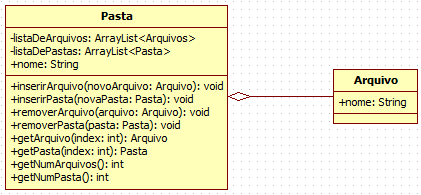
\includegraphics[scale=0.8]{composite-errado.png}
  \end{figure}

  \end{frame}

  \begin{frame}{Uma Solução}

O problema com este design é a interface que esta classe deverá ter. Como são duas listas diferentes precisaríamos de métodos específicos para tratar cada uma dela, ou seja, um método para inserir arquivos e outro para inserir pastas, um método para excluir pastas e outro para excluir arquivos, e assim vai.

Sempre que quisermos inserir uma nova funcionalidade no gerenciador precisaremos criar a mesma funcionalidade para arquivos e pastas. Além disso, sempre que quisermos percorrer uma pasta será necessário percorrer as duas listas, mesmo que vazias.

  \end{frame}

  \begin{frame}{Uma Solução}

  Bom, vamos pensar em outra solução. E se utilizássemos uma classe base Arquivo para todos os arquivos, assim precisaríamos apenas de uma lista e de um conjunto de funções. Vejamos abaixo:

  \begin{figure}
    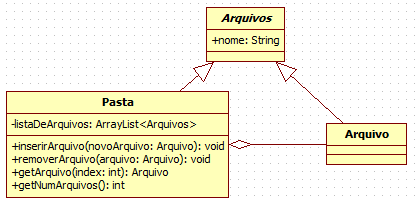
\includegraphics[scale=0.8]{composite-errado2.png}
  \end{figure}

  \end{frame}

  \begin{frame}{Uma Solução}

Pronto, resolvido o problema dos métodos duplicados. E agora, será que está tudo bem? Como faríamos a diferenciação entre um Arquivo e uma Pasta? Poderíamos utilizar o “instace of” e verificar qual o tipo do objeto, o problema é que seria necessário fazer isso SEMPRE, pois não poderíamos confiar que, dado um objeto qualquer, ele é um arquivo ou uma pasta! Sempre teríamos que fazer isso:

  \end{frame}

  \begin{frame}[fragile]
    \begin{lstlisting}{Java}
    if(arquivo instanceof Arquivo){ 
    // Codigo para tratar arquivos de video 
    } else if(arquivo instanceof Pasta){ 
    // Codigo para tratar arquivos de audio 
    }
    \end{lstlisting}

\vspace{10px}

Ok, então vamos ver uma boa solução para o problema: o padrão Composite!

  \end{frame}

\section{Composite}
\begin{frame}{Composite}

Vamos ver então qual a intenção do padrão Composite:

“Compor objetos em estruturas de árvore para representar hierarquia partes-todo. Composite permite aos clientes tratarem de maneira uniforme objetos individuais e composições de objetos.”

Bom, desta vez a intenção não está tão bem clara. A estrutura de árvore será explicada mais adiante, no momento o que interessa é a segunda parte da inteção: tratar de maneira uniforme objetos individuais.

\end{frame}

\begin{frame}{Composite}

Como o nosso problema era uniformizar o acesso aos arquivos e pastas, provavelmente o Composite seja uma boa solução.

A ideia do Composite é criar uma classe base que contém toda a interface necessária para todos os elementos e criar um elemento especial que agrega outros elementos. Vamos trazer para o nosso exemplo inicial para tentar esclarecer:

\end{frame}

\begin{frame}{Composite}
  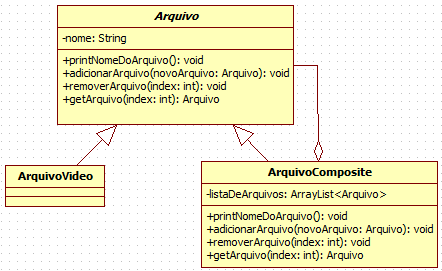
\includegraphics[scale=0.8]{composite.png}
\end{frame}

\begin{frame}{Composite}

A classe base Arquivo implementa todos os métodos necessários para arquivos e pastas, no entanto considera como implementação padrão a do arquivo, ou seja, caso o usuário tente inserir um arquivo em outro arquivo uma exceção será disparada. Veja o código da classe abaixo:

\end{frame}

\begin{frame}[fragile]

\begin{lstlisting}{Java}
public abstract class ArquivoComponent {
 
    String nomeDoArquivo;
 
    public void printNomeDoArquivo() {
        System.out.println(this.nomeDoArquivo);
    }
 
    public String getNomeDoArquivo() {
        return this.nomeDoArquivo;
    }
 
    public void adicionar(ArquivoComponent novoArquivo) throws Exception {
        throw new Exception("Nao pode inserir arquivos em: "
                + this.nomeDoArquivo + " - Nao e uma pasta");
    }

    public void remover(String nomeDoArquivo) throws Exception {
        throw new Exception("Nao pode remover arquivos em: "
                + this.nomeDoArquivo + " -Nao e uma pasta");
    }
 
    public ArquivoComponent getArquivo(String nomeDoArquivo) throws Exception {
        throw new Exception("Nao pode pesquisar arquivos em: "
                + this.nomeDoArquivo + " - Nao e uma pasta");
    }
}

\end{lstlisting}

\end{frame}

\begin{frame}[fragile]

Uma vez que tudo foi definido nesta classe, para criar um arquivo de vídeo por exemplo, basta implementar o construtor:

\begin{lstlisting}

public class ArquivoVideo extends ArquivoComponent {
 
    public ArquivoVideo(String nomeDoArquivo) {
        this.nomeDoArquivo = nomeDoArquivo;
    }
}

\end{lstlisting}

Já na classe que representa a Pasta nós sobrescrevemos o comportamento padrão e repassamos a chamada para todos os arquivos, sejam arquivos ou pastas, como podemos ver a seguir:

\end{frame}

\begin{frame}[fragile]

\begin{lstlisting}

public class ArquivoComposite extends ArquivoComponent {
 
    ArrayList<ArquivoComponent> arquivos = new ArrayList<ArquivoComponent>();
 
    public ArquivoComposite(String nomeDoArquivo) {
        this.nomeDoArquivo = nomeDoArquivo;
    }
 
    @Override
    public void printNomeDoArquivo() {
        System.out.println(this.nomeDoArquivo);
        for (ArquivoComponent arquivoTmp : arquivos) {
            arquivoTmp.printNomeDoArquivo();
        }
    }
 
    @Override
    public void adicionar(ArquivoComponent novoArquivo) {
        this.arquivos.add(novoArquivo);
    }
 
    @Override
    public void remover(String nomeDoArquivo) throws Exception {
        for (ArquivoComponent arquivoTmp : arquivos) {
            if (arquivoTmp.getNomeDoArquivo() == nomeDoArquivo) {
                this.arquivos.remove(arquivoTmp);
                return;
            }
        }
        throw new Exception("Nao existe este arquivo");
    }

\end{lstlisting}

\end{frame}

\begin{frame}[fragile]

\begin{lstlisting}
 
    @Override
    public ArquivoComponent getArquivo(String nomeDoArquivo) throws Exception {
        for (ArquivoComponent arquivoTmp : arquivos) {
            if (arquivoTmp.getNomeDoArquivo() == nomeDoArquivo) {
                return arquivoTmp;
            }
        }
        throw new Exception("Nao existe este arquivo");
    }
 
}

\end{lstlisting}

Com isto não é necessário conhecer a implementação dos objetos concretos, muito menos fazer cast. Veja como poderíamos utilizar o código do Composite:

\end{frame}

\begin{frame}[fragile]

\begin{lstlisting}

public static void main(String[] args) {
    ArquivoComponent minhaPasta = new ArquivoComposite("Minha Pasta/");
    ArquivoComponent meuVideo = new ArquivoVideo("meu video.avi");
    ArquivoComponent meuOutroVideo = new ArquivoVideo("serieS01E01.mkv");
 
    try {
        meuVideo.adicionar(meuOutroVideo);
    } catch (Exception e) {
        System.out.println(e.getMessage());
    }
 
    try {
        minhaPasta.adicionar(meuVideo);
        minhaPasta.adicionar(meuOutroVideo);
        minhaPasta.printNomeDoArquivo();
    } catch (Exception e) {
        System.out.println(e.getMessage());
    }
 
    try {
        System.out.println("\nPesquisando arquivos:");
        minhaPasta.getArquivo(meuVideo.getNomeDoArquivo())
                .printNomeDoArquivo();
        System.out.println("\nRemover arquivos");
        minhaPasta.remover(meuVideo.getNomeDoArquivo());
        minhaPasta.printNomeDoArquivo();
    } catch (Exception e) {
        e.printStackTrace();
    }
}

\end{lstlisting}

\end{frame}

\begin{frame}{Composite}

Agora podemos visualizar a tal estrutura de árvore, suponha que temos pastas dentro de pastas com arquivos, a estrutura seria parecida com a de uma árvore, veja a seguir:

\begin{figure}

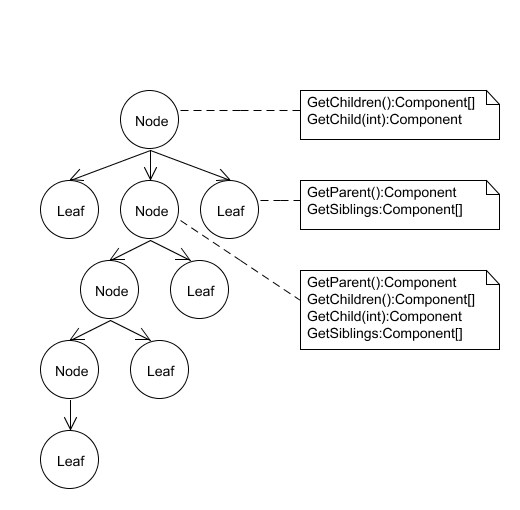
\includegraphics[height=160px]{Composite_1.jpg}

\end{figure}

\end{frame}

\begin{frame}{Composite}

Como uma estrutura de árvore temoas Nós e Folhas. No padrão Composite os arquivos concretos do nosso exemplo são chamados de Folhas, pois não possuem filhos e os arquivos pasta são chamados de Nós, pois possuem filhos e fornecem operações sobre esses filhos.

\end{frame}

\section{Conclusão}
\begin{frame}{Conclusão}

A primeira vantagem, e talvez a mais forte, seja o fato de os clientes do código Composite serem bem simplificados, pois podem tratar todos os objetos da mesma maneira. No nosso exemplo utilizei exceções para que ficasse mais evidente quando um método de uma Pasta é chamado em um Arquivo, mas suponha que os métodos não fizessem nada, a utilização seria mais simplificada ainda, pois não precisaríamos de blocos try e catch.

\end{frame}

\begin{frame}{Conclusão}

No entanto, o mal tratamento destas exceções podem gerar problemas de segurança e ai surge uma outra forma de implementar o padrão, restringindo a interface comum dos objetos. Para isto basta remover os métodos de gerenciamento de arquivos (adicionar, remover, etc) da classe base, assim apenas os arquivos pastas teriam estes métodos.

\end{frame}

\begin{frame}{Conclusão}

Em contrapartida o usuário do código precisa ter certeza se um dado objeto é Pasta para realizar um cast e chamar os métodos da pasta. 

\end{frame}

\begin{frame}{Referências}

[1] GAMMA, Erich et al. Padrões de Projeto: Soluções reutilizáveis de software orientado a objetos.

Mão na massa: Composite [https://brizeno.wordpress.com/category/padroes-de-projeto/composite/]

\end{frame}

\end{document}
